% Options for packages loaded elsewhere
\PassOptionsToPackage{unicode}{hyperref}
\PassOptionsToPackage{hyphens}{url}
%
\documentclass[
]{article}
\usepackage{lmodern}
\usepackage{amssymb,amsmath}
\usepackage{ifxetex,ifluatex}
\ifnum 0\ifxetex 1\fi\ifluatex 1\fi=0 % if pdftex
  \usepackage[T1]{fontenc}
  \usepackage[utf8]{inputenc}
  \usepackage{textcomp} % provide euro and other symbols
\else % if luatex or xetex
  \usepackage{unicode-math}
  \defaultfontfeatures{Scale=MatchLowercase}
  \defaultfontfeatures[\rmfamily]{Ligatures=TeX,Scale=1}
\fi
% Use upquote if available, for straight quotes in verbatim environments
\IfFileExists{upquote.sty}{\usepackage{upquote}}{}
\IfFileExists{microtype.sty}{% use microtype if available
  \usepackage[]{microtype}
  \UseMicrotypeSet[protrusion]{basicmath} % disable protrusion for tt fonts
}{}
\makeatletter
\@ifundefined{KOMAClassName}{% if non-KOMA class
  \IfFileExists{parskip.sty}{%
    \usepackage{parskip}
  }{% else
    \setlength{\parindent}{0pt}
    \setlength{\parskip}{6pt plus 2pt minus 1pt}}
}{% if KOMA class
  \KOMAoptions{parskip=half}}
\makeatother
\usepackage{xcolor}
\IfFileExists{xurl.sty}{\usepackage{xurl}}{} % add URL line breaks if available
\IfFileExists{bookmark.sty}{\usepackage{bookmark}}{\usepackage{hyperref}}
\hypersetup{
  pdftitle={Statistical Inference Project},
  pdfauthor={WendyD},
  hidelinks,
  pdfcreator={LaTeX via pandoc}}
\urlstyle{same} % disable monospaced font for URLs
\usepackage[margin=1in]{geometry}
\usepackage{color}
\usepackage{fancyvrb}
\newcommand{\VerbBar}{|}
\newcommand{\VERB}{\Verb[commandchars=\\\{\}]}
\DefineVerbatimEnvironment{Highlighting}{Verbatim}{commandchars=\\\{\}}
% Add ',fontsize=\small' for more characters per line
\usepackage{framed}
\definecolor{shadecolor}{RGB}{248,248,248}
\newenvironment{Shaded}{\begin{snugshade}}{\end{snugshade}}
\newcommand{\AlertTok}[1]{\textcolor[rgb]{0.94,0.16,0.16}{#1}}
\newcommand{\AnnotationTok}[1]{\textcolor[rgb]{0.56,0.35,0.01}{\textbf{\textit{#1}}}}
\newcommand{\AttributeTok}[1]{\textcolor[rgb]{0.77,0.63,0.00}{#1}}
\newcommand{\BaseNTok}[1]{\textcolor[rgb]{0.00,0.00,0.81}{#1}}
\newcommand{\BuiltInTok}[1]{#1}
\newcommand{\CharTok}[1]{\textcolor[rgb]{0.31,0.60,0.02}{#1}}
\newcommand{\CommentTok}[1]{\textcolor[rgb]{0.56,0.35,0.01}{\textit{#1}}}
\newcommand{\CommentVarTok}[1]{\textcolor[rgb]{0.56,0.35,0.01}{\textbf{\textit{#1}}}}
\newcommand{\ConstantTok}[1]{\textcolor[rgb]{0.00,0.00,0.00}{#1}}
\newcommand{\ControlFlowTok}[1]{\textcolor[rgb]{0.13,0.29,0.53}{\textbf{#1}}}
\newcommand{\DataTypeTok}[1]{\textcolor[rgb]{0.13,0.29,0.53}{#1}}
\newcommand{\DecValTok}[1]{\textcolor[rgb]{0.00,0.00,0.81}{#1}}
\newcommand{\DocumentationTok}[1]{\textcolor[rgb]{0.56,0.35,0.01}{\textbf{\textit{#1}}}}
\newcommand{\ErrorTok}[1]{\textcolor[rgb]{0.64,0.00,0.00}{\textbf{#1}}}
\newcommand{\ExtensionTok}[1]{#1}
\newcommand{\FloatTok}[1]{\textcolor[rgb]{0.00,0.00,0.81}{#1}}
\newcommand{\FunctionTok}[1]{\textcolor[rgb]{0.00,0.00,0.00}{#1}}
\newcommand{\ImportTok}[1]{#1}
\newcommand{\InformationTok}[1]{\textcolor[rgb]{0.56,0.35,0.01}{\textbf{\textit{#1}}}}
\newcommand{\KeywordTok}[1]{\textcolor[rgb]{0.13,0.29,0.53}{\textbf{#1}}}
\newcommand{\NormalTok}[1]{#1}
\newcommand{\OperatorTok}[1]{\textcolor[rgb]{0.81,0.36,0.00}{\textbf{#1}}}
\newcommand{\OtherTok}[1]{\textcolor[rgb]{0.56,0.35,0.01}{#1}}
\newcommand{\PreprocessorTok}[1]{\textcolor[rgb]{0.56,0.35,0.01}{\textit{#1}}}
\newcommand{\RegionMarkerTok}[1]{#1}
\newcommand{\SpecialCharTok}[1]{\textcolor[rgb]{0.00,0.00,0.00}{#1}}
\newcommand{\SpecialStringTok}[1]{\textcolor[rgb]{0.31,0.60,0.02}{#1}}
\newcommand{\StringTok}[1]{\textcolor[rgb]{0.31,0.60,0.02}{#1}}
\newcommand{\VariableTok}[1]{\textcolor[rgb]{0.00,0.00,0.00}{#1}}
\newcommand{\VerbatimStringTok}[1]{\textcolor[rgb]{0.31,0.60,0.02}{#1}}
\newcommand{\WarningTok}[1]{\textcolor[rgb]{0.56,0.35,0.01}{\textbf{\textit{#1}}}}
\usepackage{graphicx,grffile}
\makeatletter
\def\maxwidth{\ifdim\Gin@nat@width>\linewidth\linewidth\else\Gin@nat@width\fi}
\def\maxheight{\ifdim\Gin@nat@height>\textheight\textheight\else\Gin@nat@height\fi}
\makeatother
% Scale images if necessary, so that they will not overflow the page
% margins by default, and it is still possible to overwrite the defaults
% using explicit options in \includegraphics[width, height, ...]{}
\setkeys{Gin}{width=\maxwidth,height=\maxheight,keepaspectratio}
% Set default figure placement to htbp
\makeatletter
\def\fps@figure{htbp}
\makeatother
\setlength{\emergencystretch}{3em} % prevent overfull lines
\providecommand{\tightlist}{%
  \setlength{\itemsep}{0pt}\setlength{\parskip}{0pt}}
\setcounter{secnumdepth}{-\maxdimen} % remove section numbering

\title{Statistical Inference Project}
\author{WendyD}
\date{9/8/2020}

\begin{document}
\maketitle

\hypertarget{overview}{%
\section{Overview}\label{overview}}

In this project, we investigated the exponential distribution in R
compared to what we learned in Central Limit Theorem. We worked with 40
randomized variable and conducted 1000 stimulation. We pre-determined
lamda is 0.2

\#Simulation

\begin{Shaded}
\begin{Highlighting}[]
\KeywordTok{library}\NormalTok{(knitr)}
\end{Highlighting}
\end{Shaded}

\begin{Shaded}
\begin{Highlighting}[]
\NormalTok{n_simulation<-}\StringTok{ }\DecValTok{1000}
\NormalTok{n<-}\StringTok{ }\DecValTok{40}
\NormalTok{lambda<-}\StringTok{ }\FloatTok{0.2}
\NormalTok{rep<-}\KeywordTok{rexp}\NormalTok{(n}\OperatorTok{*}\NormalTok{n_simulation, }\FloatTok{0.2}\NormalTok{)}
\end{Highlighting}
\end{Shaded}

Inputing the result into a matrix for easier manipulation

\begin{Shaded}
\begin{Highlighting}[]
\NormalTok{data<-}\StringTok{ }\KeywordTok{matrix}\NormalTok{(rep, n_simulation, n)}
\end{Highlighting}
\end{Shaded}

\hypertarget{sample-mean-and-theoretical-mean}{%
\section{Sample Mean and Theoretical
mean}\label{sample-mean-and-theoretical-mean}}

Theoretical Mean

\begin{Shaded}
\begin{Highlighting}[]
\NormalTok{theoretical_mean<-}\DecValTok{1}\OperatorTok{/}\NormalTok{lambda}
\end{Highlighting}
\end{Shaded}

Sample Mean For each simulation (Row), we calculated the mean

\begin{Shaded}
\begin{Highlighting}[]
\NormalTok{sim_mean<-}\KeywordTok{rowMeans}\NormalTok{(data)}
\NormalTok{sample_mean<-}\StringTok{ }\KeywordTok{mean}\NormalTok{(sim_mean)}
\end{Highlighting}
\end{Shaded}

Making a data.frame for easier comparision

\begin{Shaded}
\begin{Highlighting}[]
\KeywordTok{data.frame}\NormalTok{(theoretical_mean, sample_mean)}
\end{Highlighting}
\end{Shaded}

\begin{verbatim}
##   theoretical_mean sample_mean
## 1                5    5.011975
\end{verbatim}

We see that that the sample mean is pretty close to theoretical mean
(4.9544 vs 5)

It would be helpful to plot the distribution of the mean over a
histogram plot, then input two line representing sample mean(blue) and
our theoretical mean(in Red)

\begin{Shaded}
\begin{Highlighting}[]
\KeywordTok{library}\NormalTok{(ggplot2)}
\end{Highlighting}
\end{Shaded}

\begin{Shaded}
\begin{Highlighting}[]
\NormalTok{sim_meanframe<-}\StringTok{ }\KeywordTok{as.data.frame}\NormalTok{(sim_mean)}
\KeywordTok{ggplot}\NormalTok{(}\DataTypeTok{data=}\NormalTok{sim_meanframe, }\KeywordTok{aes}\NormalTok{(}\DataTypeTok{x=}\NormalTok{ sim_mean))}\OperatorTok{+}
\StringTok{       }\KeywordTok{geom_histogram}\NormalTok{(}\DataTypeTok{position=}\StringTok{"identity"}\NormalTok{, }\DataTypeTok{colour=}\StringTok{"black"}\NormalTok{)}\OperatorTok{+}
\StringTok{       }\KeywordTok{xlab}\NormalTok{(}\StringTok{"Sample mean"}\NormalTok{) }\OperatorTok{+}\StringTok{ }\KeywordTok{geom_vline}\NormalTok{(}\DataTypeTok{xintercept =}\NormalTok{ sample_mean, }\DataTypeTok{colour=}\StringTok{"blue"}\NormalTok{)}\OperatorTok{+}
\StringTok{       }\KeywordTok{geom_vline}\NormalTok{(}\DataTypeTok{xintercept =}\NormalTok{ theoretical_mean, }\DataTypeTok{colour=}\StringTok{"red"}\NormalTok{)}
\end{Highlighting}
\end{Shaded}

\begin{verbatim}
## `stat_bin()` using `bins = 30`. Pick better value with `binwidth`.
\end{verbatim}

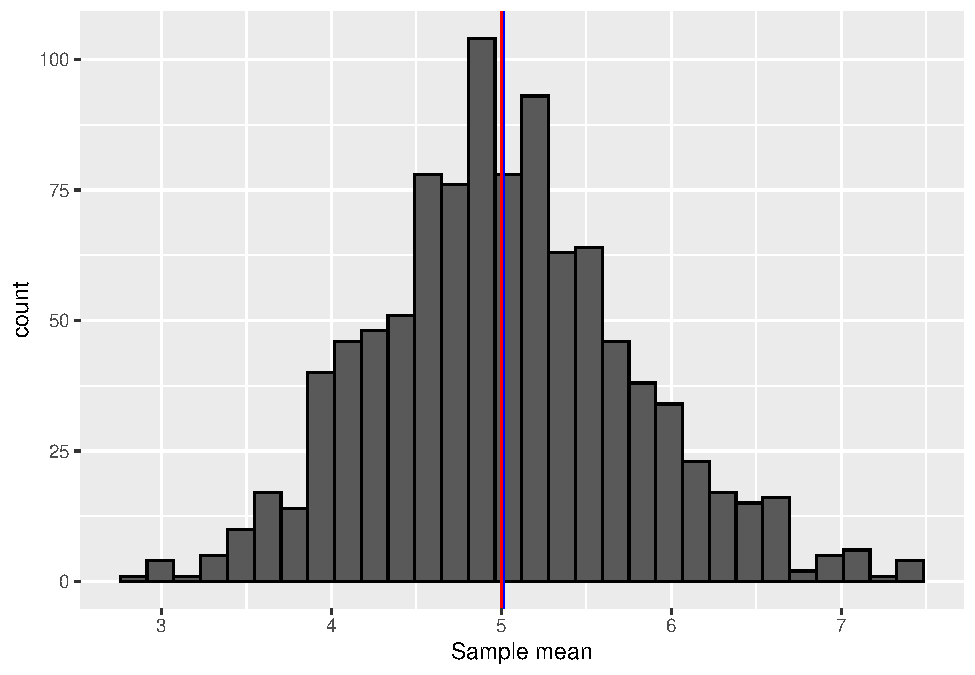
\includegraphics{StatisticalInference_Project_Week4_files/figure-latex/unnamed-chunk-8-1.pdf}

\hypertarget{theoretical-variance-vs-sample-variance}{%
\section{Theoretical Variance vs Sample
Variance}\label{theoretical-variance-vs-sample-variance}}

We first begin by computing the variance from our actual sample, and
theoretical variance:

\begin{Shaded}
\begin{Highlighting}[]
\NormalTok{sample_var<-}\StringTok{ }\KeywordTok{var}\NormalTok{(sim_mean)}
\NormalTok{theoretical_var<-}\StringTok{ }\NormalTok{(}\DecValTok{1}\OperatorTok{/}\NormalTok{lambda)}\OperatorTok{^}\DecValTok{2}\OperatorTok{/}\NormalTok{n}
\end{Highlighting}
\end{Shaded}

Making a data.frame for easier comparision

\begin{Shaded}
\begin{Highlighting}[]
\KeywordTok{data.frame}\NormalTok{(theoretical_var,sample_var)}
\end{Highlighting}
\end{Shaded}

\begin{verbatim}
##   theoretical_var sample_var
## 1           0.625  0.5801578
\end{verbatim}

The sample variance is 0.5999 while theoretical variance is 0.625. These
two values are close.

\#Distribution

We want to compare our data distribution with the distribution from
central limit theorem. According to CLT, the average of our sample will
follow normal distribution.

We first plot our data and a density curve to see if our data align with
the normal distribution

\begin{Shaded}
\begin{Highlighting}[]
\KeywordTok{ggplot}\NormalTok{(}\DataTypeTok{data=}\NormalTok{sim_meanframe, }\KeywordTok{aes}\NormalTok{(}\DataTypeTok{x=}\NormalTok{sim_mean))}\OperatorTok{+}
\StringTok{       }\KeywordTok{geom_histogram}\NormalTok{(}\KeywordTok{aes}\NormalTok{(}\DataTypeTok{y =} \KeywordTok{after_stat}\NormalTok{(density)), }\DataTypeTok{position=}\StringTok{"identity"}\NormalTok{, }\DataTypeTok{colour=}\StringTok{"black"}\NormalTok{)}\OperatorTok{+}
\StringTok{       }\KeywordTok{xlab}\NormalTok{(}\StringTok{"Sample mean"}\NormalTok{)}\OperatorTok{+}
\StringTok{        }\KeywordTok{ggtitle}\NormalTok{(}\StringTok{"Sample mean distribution with density curve"}\NormalTok{)}\OperatorTok{+}
\StringTok{        }\KeywordTok{geom_density}\NormalTok{(}\DataTypeTok{colour=}\StringTok{"blue"}\NormalTok{, }\DataTypeTok{size=}\DecValTok{2}\NormalTok{)}
\end{Highlighting}
\end{Shaded}

\begin{verbatim}
## `stat_bin()` using `bins = 30`. Pick better value with `binwidth`.
\end{verbatim}

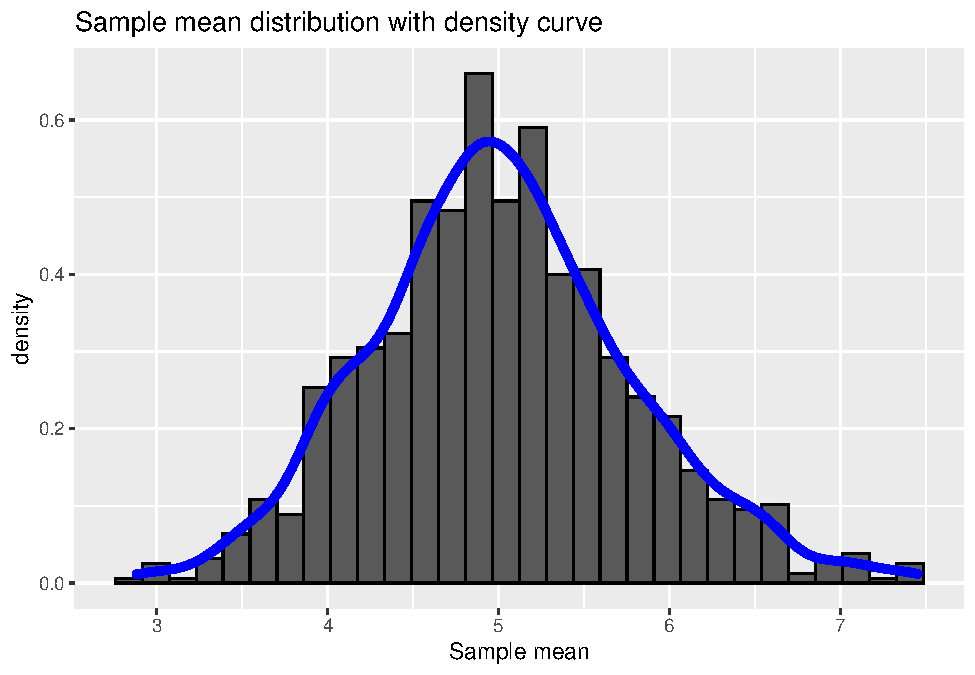
\includegraphics{StatisticalInference_Project_Week4_files/figure-latex/unnamed-chunk-11-1.pdf}

We now have compared the theoretical mean vs sample mean, theoretical
variance vs sample variance. We will investigate the last element:
confidence interval

\begin{Shaded}
\begin{Highlighting}[]
\NormalTok{sample_conf_interval <-}\StringTok{ }\KeywordTok{round}\NormalTok{ (}\KeywordTok{mean}\NormalTok{(sim_mean) }\OperatorTok{+}\StringTok{ }\KeywordTok{c}\NormalTok{(}\OperatorTok{-}\DecValTok{1}\NormalTok{,}\DecValTok{1}\NormalTok{)}\OperatorTok{*}\FloatTok{1.96}\OperatorTok{*}\KeywordTok{sd}\NormalTok{(sim_mean)}\OperatorTok{/}\KeywordTok{sqrt}\NormalTok{(n),}\DecValTok{3}\NormalTok{)}


\NormalTok{theoretical_conf_interval <-}\StringTok{ }\NormalTok{theoretical_mean}\OperatorTok{+}\StringTok{ }\KeywordTok{c}\NormalTok{(}\OperatorTok{-}\DecValTok{1}\NormalTok{,}\DecValTok{1}\NormalTok{)}\OperatorTok{*}\FloatTok{1.96}\OperatorTok{*}\KeywordTok{sqrt}\NormalTok{(theoretical_var)}\OperatorTok{/}\KeywordTok{sqrt}\NormalTok{(n)}
\end{Highlighting}
\end{Shaded}

The actual 95\% confidence interval is \texttt{sample\_conf\_interval}
and the theoretical confidence interval
\texttt{theoretical\_conf\_interval} are pretty close to one another
also

Lastly, we used qqplot to draws the correlation between a given sample
and the normal distribution. If the data is normally distributed, the
points in the QQ-normal plot lie on a straight diagonal line

\begin{Shaded}
\begin{Highlighting}[]
\KeywordTok{qqnorm}\NormalTok{(sim_mean, }\DataTypeTok{pch =} \DecValTok{1}\NormalTok{, }\DataTypeTok{frame =} \OtherTok{FALSE}\NormalTok{)}
\KeywordTok{qqline}\NormalTok{(sim_mean,}\DataTypeTok{col =}\StringTok{"2"}\NormalTok{,}\DataTypeTok{lwd =} \DecValTok{2}\NormalTok{)}
\end{Highlighting}
\end{Shaded}

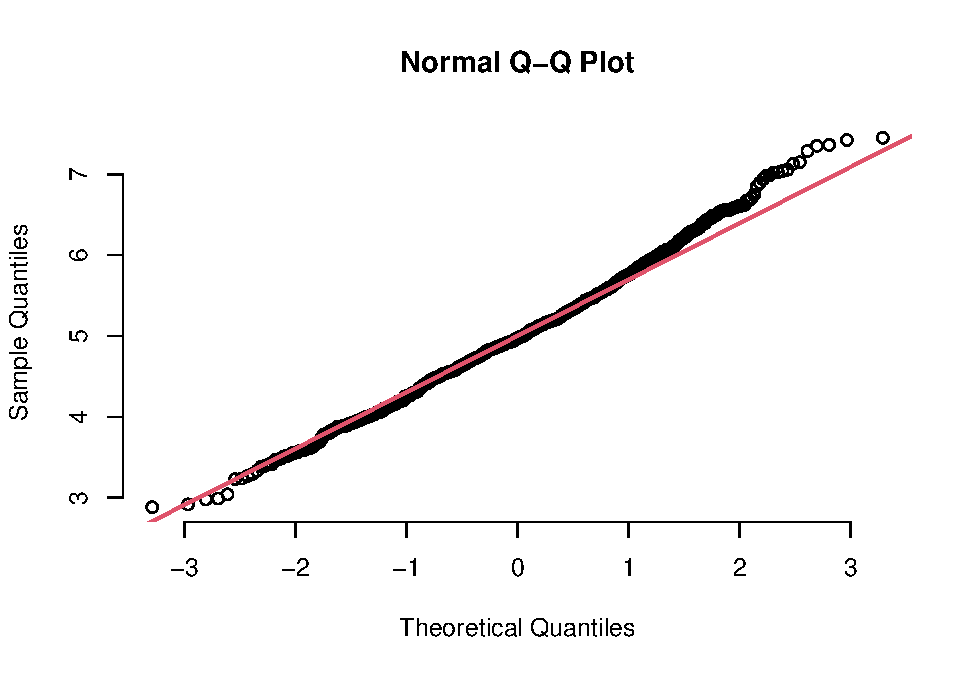
\includegraphics{StatisticalInference_Project_Week4_files/figure-latex/unnamed-chunk-13-1.pdf}

The difference between the dots and the line is minimal. Thus we can
conclude that the sample is relatively normally distributed.

\end{document}
